\section{Design}
\label{s:design}
\hspace{10pt} This section describes the design of the software components and the experiments involved in the dissertation. The first subsection outlines how energy demands of different sensors are compared. This includes the design principles behind sample sensor applications and the details on how to measure their energy efficiency. The second subsection layouts the energy-efficient sensing library, Locy. It summarizes its energy-efficient algorithm, how the algorithm can be differentiated depending on the battery life and the library's architecture. The design presented in this section will be revisited in the next section.

\subsection{Sensor energy measurements}
\label{s:design:measurements}
\hspace{10pt} Sensor energy measurements is a part of the project, where the energy efficiency of different sensors are determined. To achieve this objective, each sensor is represented in the series of simple Android applications, \textbf{Sample Sensor Applications}. Each of those applications keeps continuously sampling one sensor and switches off all others. Sample Sensor Applications are designed in the way that only one difference between them should be which sensor is being currently sampled. To compare sensors' energy demands, the novel method of measuring energy efficiency of the applications is proposed. The method calculates time which each application needs to deplete one percentage of battery life. The order of energy efficiency of different sensors may be established by comparing those time measurements: the most energy efficient sensor will be the one which one percentage battery depletion takes the longest. 

\subsubsection{Sample sensor applications}
\label{s:design:measurements:sampleapps}
\hspace{10pt} To determine differences in sensors' energy efficiency, each of sample applications keeps sampling only one sensor while all others sensors are being switched off.  However, \textbf{this triggers other differences between applications}: various sampling frequencies and size of sensor data. Sine I aim to compare the energy efficiency of sampling itself, those other differences' impact is trying to be minimized. 

\textbf{Sampling frequencies vary among sensors}. Inertial sensors e.g., accelerometer or gyroscope could be sampled as often as every 20 milliseconds, whereas the minimum frequency of GPS equals to 20 seconds. The issue is more complex in case of wireless communication sensors such as Bluetooth or IEEE 802.11. A full Bluetooth scan takes around 12 secs, but it could be stopped earlier and started again. To alleviate those differences, \textbf{the least energy-efficient strategy of complete, correct sampling} is chosen for the comparison of sensors' energy efficiency. Sensors are being sampled as often as possible providing that the previous sample delivered valid data. For example, the next IEEE 802.11 scan will be started once the previous one has been finished\ (IEEE 802.11 scan takes around 2.5 secs depending on the device). This provides complete information on available access points while minimizing sampling frequency, which increases its energy consumption. The strategy will look similar for GPS and Bluetooth. In case of other sensors (inertial sensors, camera and microphone), the strategy will be executed by sensors being sampled as often as possible (sampling is immediate). 

To check whether Sample Sensor Applications work correctly, each application prints out its raw sensor data. The frequency of this output equals to 1 second and is the same for all applications. As described in the previous paragraph, sensors data are delivered on different frequencies. If the raw data would be also printed on different frequencies, this could add noise to our experiments. By using \textbf{the same frequency of printing out raw data for all applications}, the differences in sampling frequencies are mitigated. GPS sample application will print out its raw sensor data as often as accelerometer sample application, though those applications have different sensor sampling frequencies. It is worth noticing that as a side effect, printed values may be repetitive or missing, when no new sensor data were delivered. 

Another issue concerning application's output is \textbf{different sizes of raw data among sensors}. For example, the result of wireless communication scans\ (IEEE 802.11 and Bluetooth) is the list of records (e.g., 20 hot spots with their names and other parameters), whereas light sensor's result  is just a single number. Furthermore, more complex data is delivered by camera or microphone. As the raw data is printed on regular basis, those differences could lead to significant changes in energy efficiency of Sample Sensor Applications. To alleviate those differences, \textbf{the output is standardized} and has the same form for all applications. The one line of the output, which includes between 1 and 3 numbers, is printed.

Those number may represent different information depending on a sensor:
\begin{itemize}
	\item For wireless communications sensors, only the amount of available hotspot/devices is printed: 
		\plot{output_wifiscan}
	\item For microphone, the maximum absolute amplitude for every second is printed:
		\plot{output_microphone}
	\item For camera, the total size of recorder video is printed:
		\plot{output_camera}
	\item Light and proximity sensor provide only one value:
		\plot{output_light}
	\item Other inertial sensor provide all three coordinates:
		\plot{output_inertial}
\end{itemize}

There are still other issues, which could add noise to the experiments e.g., various API among sensors or different capabilities of IEEE 802.11 wireless cards. However, all differences noticeable on the application level are eliminated. Such design of Sample Sensor Applications guarantees that on the energy efficiencies of different sensors' sampling will be compared. 
				
\subsubsection{1\% battery depletion}	
\label{s:design:measurements:method}
\hspace{10pt} Once  Sample Sensor Applications are prepared, the order of their energy efficiency needs to be established. To compare their energy efficiency, time measurements on how long 1\% depletion of battery life takes are made. Then, those time measurements are compared. For any two sensors, if there is longer time needed for 1\% depletion of one of them, it means that this sensor is more energy-efficient. It is worth mentioning that 1\% is used, since that is a precision of the information on battery life's status which Android API provides.

\textbf{The method should be accurate if the comparison is made on the same percentage of battery life} e.g., between 99\% and 98\%. Although the battery life is nonlinear, the battery should behave similarly on the same percentage across many runs. The measurements should be similar and repetitive. Also, time measurements should not take long, which creates a chance for accurate online energy measurements. All of those assumptions will be validated in the next section.

For the purpose of this dissertation, this measurement method was directly incorporated into Sample Sensor Applications. Each sample sensor application is continuously querying the battery status and the time of 1\% battery depletion is registered. The whole process is exactly the same for all sample sensor applications. Because of that, no noise to the experiments is added.

\subsubsection{The list of sample sensor applications}	
\label{s:design:measurements:applications}
\hspace{10pt} The Table \ref{table:samplesensorapps} consists of the complete list of Sample Sensor Applications created for this project. Beside the Sample Sensor Applications, a couple of supporting applications were implemented:
\begin{itemize}
	\item EnergyMeasurementListSensors - listing all physical sensors available in a mobile phone.
	\item EnergyMeasurementNetwork - determining energy efficiency of Android wireless-based localization.
	\item EnergyMeasurementGPSSatellites - determining energy efficiency of acquiring GPS Satellites' signal without solving navigation equations on a mobile phone.	
\end{itemize}
All of those applications could be found in \textit{sensors\_energy\_measurement/sample\_apps} directory.
		
\begin{table}[H]
	\centering
    \begin{tabular}{| l | r | }
    \hline
    \textbf{Sensor} & \textbf{Application name} \\ \hline
    Camera & EnergyMeasurementCamera \\ \hline
    Microphone & EnergyMeasurementMicrophone \\\hline
    IEEE 802.11 & EnergyMeasurementWifi80211 \\ \hline
    GPS & EnergyMeasurementGPS \\ \hline
    Bluetooth & EnergyMeasurementBluetooth \\ \hline
    Bluetooth LTE & EnergyMeasurementBluetoothLE \\ \hline
    Accelerometer & EnergyMeasurementAcceleromter \\ \hline
    Gyroscope & EnergyMeasurementGyroscope \\ \hline
    Magnetic Field & EnergyMeasurementMagneticField\\ \hline
    Ambient Light & EnergyMeasurementLight \\ \hline
    Proximity & EnergyMeasurementProximity \\ \hline
    \end{tabular}
    \caption{The complete list of Sample Sensor Applications.}
	\label{table:samplesensorapps}
\end{table}			


\subsection{Locy}
\label{s:design:locy}
\hspace{10pt}Locy is an energy-efficient sensing library for Android phones. It utilizes the idea of a relation between sensors to provide energy-efficient localization for mobile applications. The relation is between accelerometer and GPS sensors. The former sensor may be user to check whether a user is moving or not. If a user is not moving, his geographical location does not change\ (his GPS coordinates do not change). Therefore, GPS sampling may be switched off. This operation will bring energy savings, since GPS sampling has higher energy demands than accelerometer does. 

There are three important features in the library, which require further explanation. First, a moving detection algorithm needs to be carefully designed to accurately check whether a user is moving. Second, this algorithm needs to be energy-efficient itself. This goal is achieved by duty-cycling sampling and its dependent on the battery life of a device\ (the Requirement \ref{r:library:adaptive}). Lastly, the software infrastructure of the library needs to be further discussed. Since the library is aimed at being plugged to existing applications\ (the Requirement \ref{r:library:esm}), its API needs to satisfy specific needs. 

\subsubsection{Moving detection algorithm}
\label{s:design:locy:moving}
\hspace{10pt}The moving detection algorithm is based on accelerometer sensor. The sensor provides the raw data describing the acceleration of a device in three dimensions\ (x, y, z relatively to the position of a device).  The data is difficult to analyze: the acceleration of a user may be split between the axes in different ways depending on the initial position of a mobile phone. While a user is walking, accelerometer data will be significantly different depending on where a user is keeping his mobile phone\ (horizontally in a purse or vertically in trousers pocket). To simplify the analysis, \textbf{the total magnitude} is applied over accelerometer data\ (Equation \ref{e:total_magnitude}). This reduces the dimension of the data to one and still has the information on the acceleration of a user. 

\begin{equation}\label{e:total_magnitude}
total\;magnitude = x^2 + y^2 + z^2
\end{equation}

Once the total magnitude over accelerometer data is applied, the accelerometer readings of a user's walking and his staying in one place may be compared\ (the Figure \ref{p:moving:magnitude}). A user's walking may be characterized by \textbf{the series of peaks}. A user makes a step by lifting up his foot and putting it back on the ground. His another foot moves in similar patterns. A peak on a graph corresponds to a user's step. If a user is in place, there are no peaks observed. 

\begin{figure}[H]
\centering
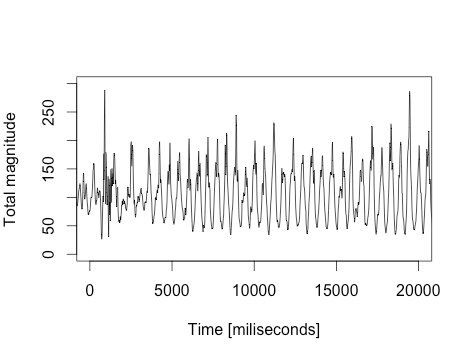
\includegraphics[width=0.49\textwidth, scale=0.6]{plots/walking}
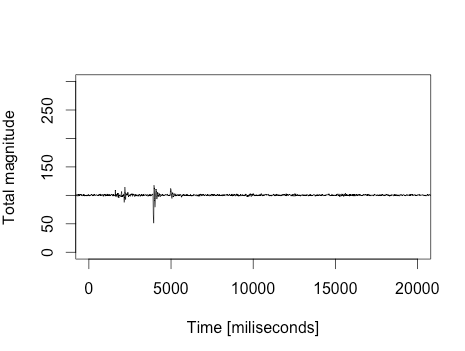
\includegraphics[width=0.49\textwidth, scale=0.6]{plots/no_walking}
\caption{\label{p:moving:magnitude} The difference in total magnitude over accelerometer data between walking and not walking. Walking may be characterized by the series of peaks. One peak corresponds to  a step made by a user.}
\end{figure}

For the purpose of Locy, the difference between walking and staying in one place needs to be formalized. While a user is walking, the series of peaks means the high variation of the accelerometer data, which can be expressed by \textbf{standard deviation}. The Figure \ref{p:moving:stddev} contrasts the standard deviation while a user is walking and not\ (a standard deviation was calculated over 2.5 seconds intervals). It can be noticed that the standard deviation is much bigger when a user is walking.

\begin{figure}[H]
\centering
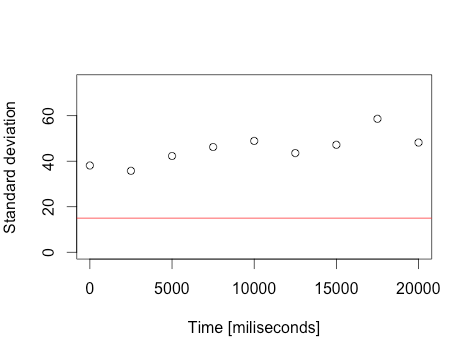
\includegraphics[width=0.49\textwidth, scale=0.6]{plots/stddev_walking}
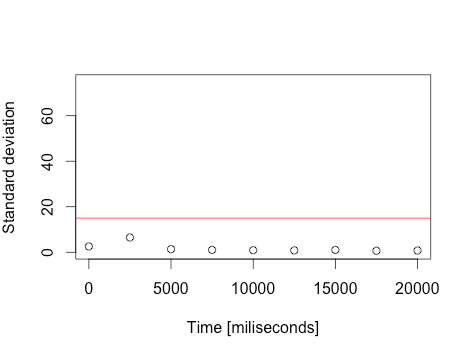
\includegraphics[width=0.49\textwidth, scale=0.6]{plots/stddev_no_walking}
\caption{\label{p:moving:stddev} The difference in standard deviation over total magnitude of accelerometer data between walking and not walking. Walking is characterized by higher standard deviation. The threshold of 15 is chosen to classify a user's movement.}
\end{figure}

There are two challenges in this approach. First, the duration of sampling windows\ (the interval over which a standard deviation is calculated) needs to be chosen. The Figure \ref{p:moving:stddev} uses 2.5 seconds as the duration of sampling windows. Second, the threshold of standard deviation for the movement classification needs to be determined. The Figure \ref{p:moving:stddev} defines the threshold as 15. Both of those parameters were determined in a \textbf{trial-and-error} approach. Different values were chosen and evaluated against the small data set collected for the purpose of this project. The best accuracy was provided by the parameters used in the Figure \ref{p:moving:stddev} i.e. 2.5 seconds for sampling windows and 15 as the threshold for movement classification. The details of the trial-and-error approach are presented in the section \ref{s:implementation:moving}.

Locy provides the accurate movement detection by undertaking the classification over three consecutive sampling windows. It at least two of them indicates that a user is walking\ (the standard deviation is above the threshold), then a user activity is classified as walking. Three consecutive sampling windows last in total 7.5 seconds\ (the duration of the sampling window is 2.5 seconds). It is assumed that such a movement detection algorithm is accurate and should be universal i.e. it does not dependent on a type of mobile phone, its position or a user.

\subsubsection{Adaptive duty-cycling sampling}
\label{s:design:locy:adaptive}
\hspace{10pt}A user is not likely to change its activity\ (moving or not) every 8 seconds. This observation could be leveraged for energy optimization. Instead of continuous accelerometer sampling and the movement classification, the device could sleep for the certain period of time and conserve an energy. After this sleeping interval, the device could start sampling again. This approach is called \textbf{duty-cycling} and is incorporated in Locy. 

Duty-cycling sampling may be customized by changing its \textbf{duty-cycling ratio} between the duration of sampling windows and sleeping intervals. For example, the ratio equaled to 0.5 means that the duration of sampling windows is twice smaller than the duration of sleeping intervals. There is a \textbf{energy-accuracy trade-off} in choosing the ratio. If the ratio is smaller, the important events are more likely to be missed as sampling windows are relatively shorter. On the other hand, smaller ratio leads to bigger energy optimization as the sleeping intervals are relatively longer. The trade-off is utilized by Locy, which changes its duty-cycling ratio depending on \textbf{the battery life} of a device. If the level of battery life is high, the duty-cycling ratio is also high. In that case, Locy does not miss any important events, but may not be the most energy-efficient. If the level of battery level decreases, Locy also decreases its duty-cycling ratio, which leads to additional energy savings. Such approach satisfies one of the project's secondary requirements\ (the Requirement \ref{r:library:adaptive}). The details on how the ratio changes are presented in the Table \ref{table:locy:dutycyclingratio}.

\begin{table}[H]
	\centering
    \begin{tabular}{| c | c | }
    \hline
    Battery life & Duty-cycling ratio \\ \hline
    80-100\% & 1 \\ \hline
    60-80\% & 0.5\\ \hline
    40-60\% & 0.33\\ \hline
    20-40\% & 0.25\\ \hline
    0-20\% & 0.2 \\ \hline
    \end{tabular}
    \caption{The different duty-cycling ratios in Locy depending on the battery life of a device. Locy adopts its algorithm depending on a current battery life. }
	\label{table:locy:dutycyclingratio}
\end{table}	

\subsubsection{Software architecture}
\label{s:design:locy:architecture}
\hspace{10pt}Locy is an Android library project, which is intended to be plugged into the existing applications. Most of those applications use localization services provided by Android's LocationManager. Developers wishing replacing LocalizationManager with Locy should not have much difficulties. Locy API is consistent with LocationManager API. A developer only needs to add Locy library to its existing project and change one line in his source code: instead of getting LocationManager\ (Listing\ref{ls:locationmanager}), LocyManager needs to be created\ (Listing \ref{ls:locymanager}). All other parts of the code should work perfectly without any additional changes. This approach was tested by plugging Locy in Tristan's Experience Sampling Method\ (ESM) mobile application. This primary requirement\ (the Requirement \ref{r:library:esm}) was achieved without any difficulties and its result may be viewed in the \textit{ESM/} directory.

                 
\begin{lstlisting}[language=Java,
       basicstyle=\ttfamily,
       keywordstyle=\color{blue}\ttfamily,
       stringstyle=\color{red}\ttfamily,
       commentstyle=\color{green}\ttfamily,
      breaklines=true,
      frame=single,    
      label=ls:locationmanager,caption=Localization services with LocationManager.]
LocationManager locationManager =  (LocationManager) getSystemService(LOCATION_SERVICE);
\end{lstlisting}

\begin{lstlisting}[language=Java,
       basicstyle=\ttfamily,
       keywordstyle=\color{blue}\ttfamily,
       stringstyle=\color{red}\ttfamily,
       commentstyle=\color{green}\ttfamily,
      breaklines=true,
      frame=single,    
      label=ls:locymanager,caption=Localization services with LocyManager.]
LocyManager locationManager = new LocyManager(this);
\end{lstlisting}

